\documentclass[a4paper]{article}

\usepackage{color}
\usepackage{url}
\usepackage[T2A]{fontenc} 
\usepackage[utf8]{inputenc}
\usepackage{graphicx}

\usepackage[english,serbian]{babel}
\usepackage[unicode]{hyperref}
\hypersetup{colorlinks,citecolor=red,filecolor=green,linkcolor=blue,urlcolor=blue}

\title{IS_Firme}
\date{November 2023}

\begin{document}

\begin{titlepage}
    \centering

    \newcommand{\HRule}{\rule{\linewidth}{0.5mm}}
    \center
    \textup{\Large Univerzitet u Beogradu\\Matematički fakultet}\\[1.5cm]
    \textup{\Large Projekat iz predmeta Informacioni sistemi 2022/2023.}\\[0.4cm]

    \HRule \\[0.4cm]
    { \huge \bfseries Informacioni sistem firme}\\[0.4cm]
    \HRule \\[1.1cm]
\end{titlepage}

\newpage
\renewcommand*\contentsname{Sadržaj:}
\tableofcontents

\newpage
\section{Analiza sistema}
\subsection{Uvod i osnovna ideja}
Ideja projekta je pravljenje informacionog sistema koji bi se koristio za vođenje evidencije o zaposlenima u jednoj programerskoj firmi. Ono što to podrazumeva je beleženje radnog vremena, beleženje odmora i slobodnih dana, rada od kuće, kao i informacije o benefitima čije troškove pokriva firma.

\subsection{Korisnici sistema}
Korisnici sistema su:
\begin{enumerate}
    \item \textbf{Zaposleni} \newline
    Zaposleni su najbrojniji korisnici sistema. Svakom zaposlenom je dodeljen tim kome on pripada, zaposleni može da menja timove. Funkcionalnosti koje će sistem pružiti radnicima je prijavljivanje ostvarenog radnog vremena, prijavljivanje odmora, podnošenje zahteva za rad od kuće i podnošenje zahteva za korišćenje benefita.
    \item \textbf{Vođa tima} \newline
    Vođa tima upravlja timom koji mu je dodeljen, on je i sam zaposleni. U svakom trenutku mu se njegovom timu može dodeliti novi član. Funkcionalnosti koje sistem pruža vođi tima su odobravanje zahteva zaposlenog, kreiranje zahteva za re-evaluaciju zaposlenog, zahtev za korišćenje benefita za nekog zaposlenog.
    \item \textbf{Menadžer ljudskih resursa} \newline 
    Menadžer ljudskih resursa je zadužen za evidentiranje informacija koje su bitne za sve zaposlene. Funkcionalnosti koje sistem pruža menadžeru za ljudske resurse su obračun plata, unos važnih datuma i dodela odobrenih benefita i bonusa.
    \item \textbf{Administrator} \newline
    Administrator je zadužen za odrzavanje sistema. Njegove dužnosti tokom korišćenja sistema su kreiranje naloga zaposlenima, brisanje naloga ljudima koji su prekinuli radni odnos, omogućavanje ponovnog pristupa nalogu pri zahtevu zaposlenog i obezbeđivanje opreme za rad. 
\end{enumerate}

\subsection{Udruženja}
Udruženja predstavljaju entitet unutar informacionog sistema, kome se pridružuju zaposleni koji dele zajednički interes. \newline
Informacioni sistem obezbedjuje zasebnu stranicu koja pripada udruženju, koja se može koristiti povodom:
\begin{enumerate}
    \item Diskusija u okviru domena interesa udruženja.
    \item Deljenja informacija i znanja među članovima.
    \item Organizovanje događaja.
\end{enumerate}

Za osobu zaposlenu u kompaniji, bez obzira na ulogu u okviru iste, važe sledeća pravila u okvriu informacionog sistema:
\begin{itemize}
    \item Dozvoljeno je kreiranje udruženja, uz odgovarajuće odobrenje od strane menadžera ljudskih resursa.
    \item Dozvoljeno je članstvo u proizvoljnom broju udruženja.
    \item Dozvoljeno je kreiranje događaja, uz odgovarajuće odobrenje od strane kreatora (vlasnika) udruženja.
\end{itemize}

\newpage
\section{Slučajevi upotrebe}

\subsection{Aktivnosti Administratora}

\begin{figure} [!ht]
    \begin{center}
        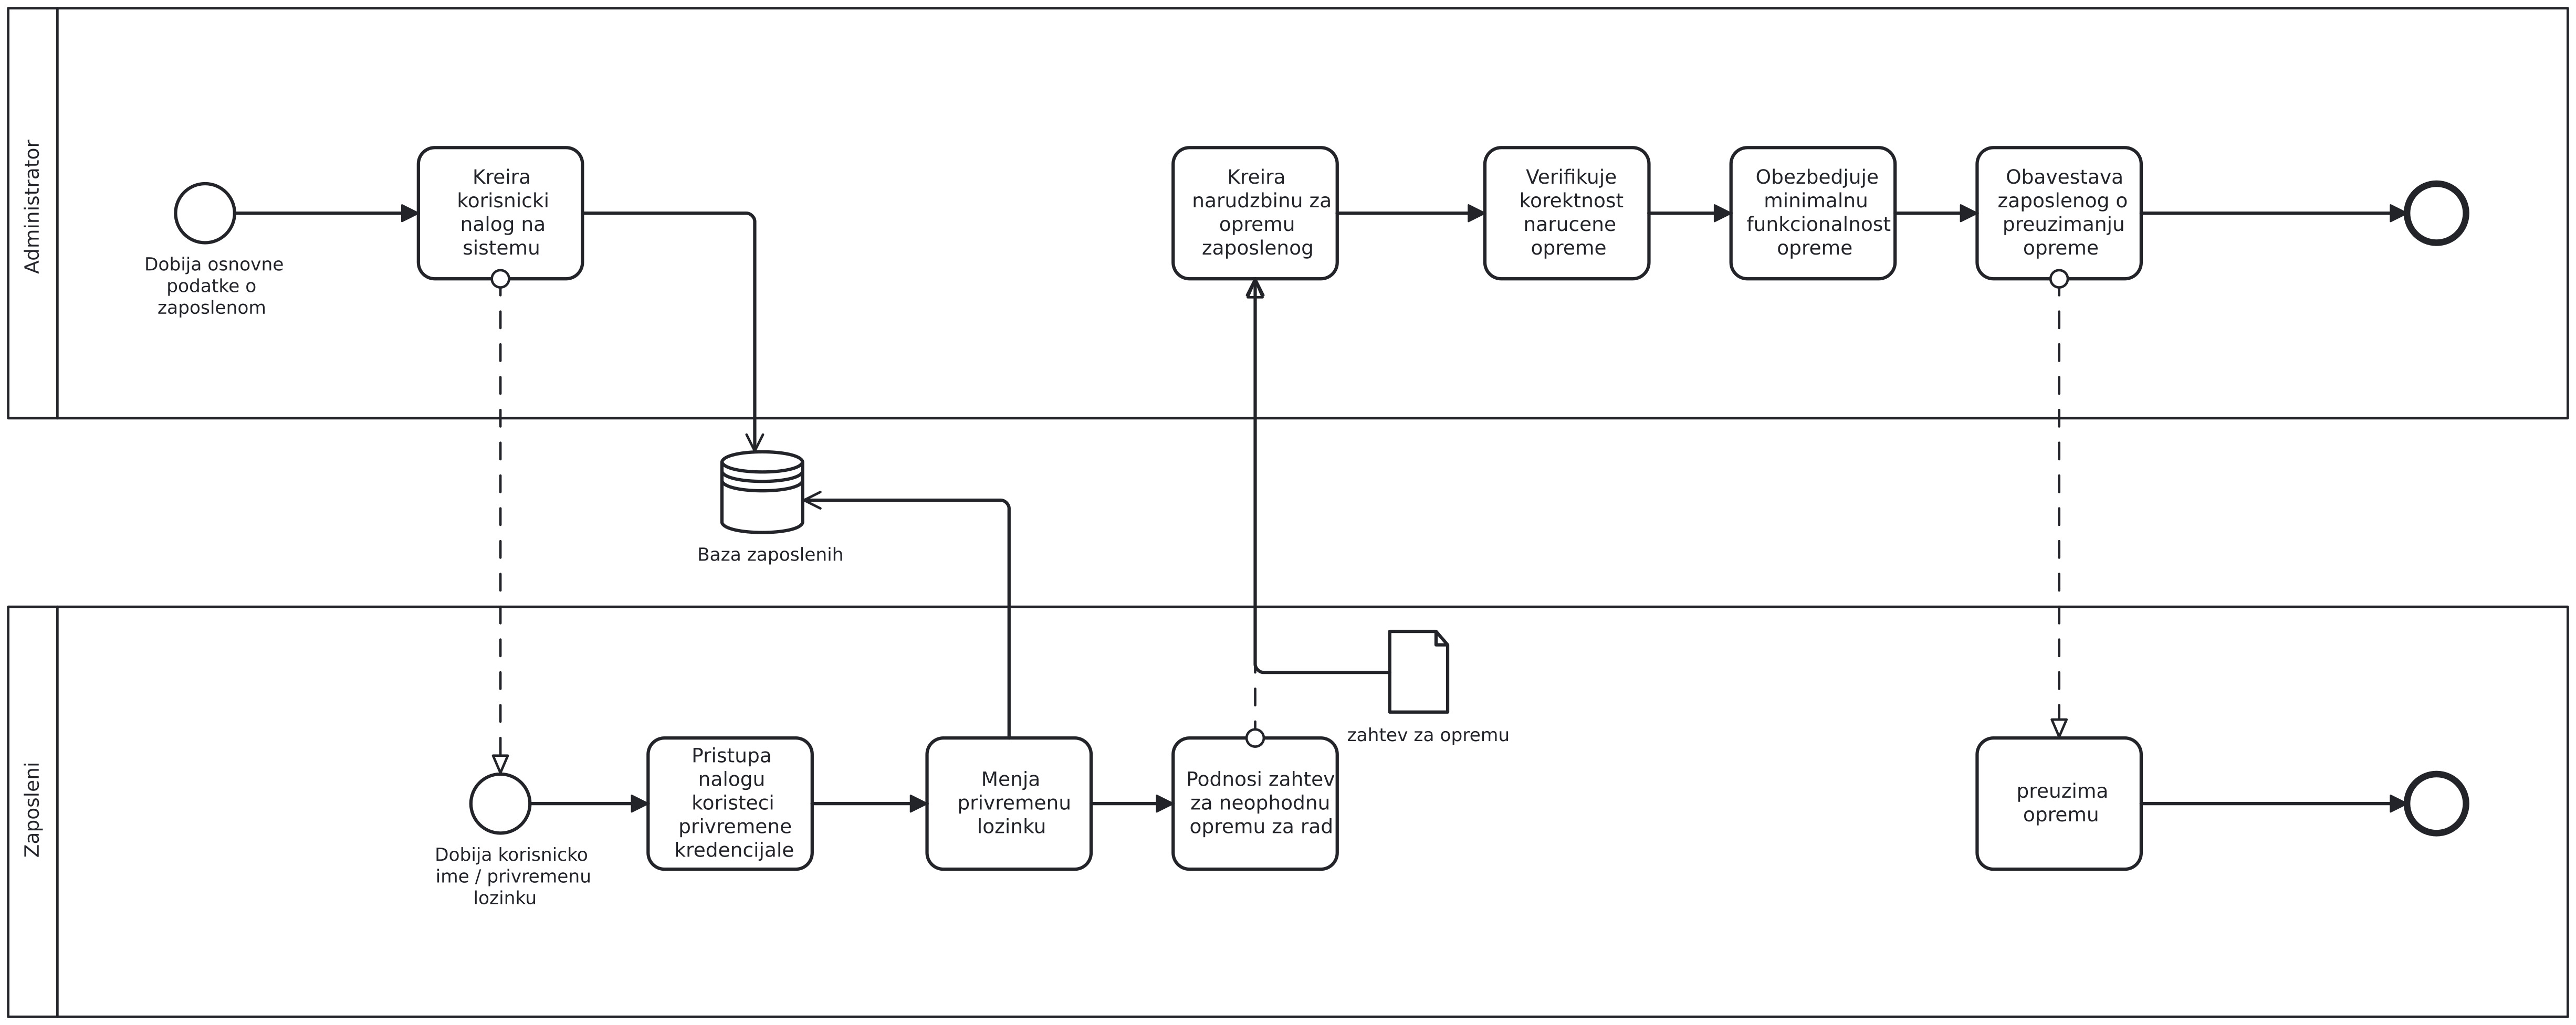
\includegraphics[width=\textwidth,height=\textheight,keepaspectratio]{{Korisnici/Administrator/BPMN/onboarding.jpg}}
    \end{center}
\caption{Dijagram procesa omogućavanja pristupa sistemu i opremanja novog zaposlenog}
\end{figure}

\subsubsection{Slučaj upotrebe: Kreiranje naloga zaposlenom}
\begin{enumerate}
    \item \textbf{Kratak opis:} Administrator kreira nalog zaposlenoj osobi u kompaniji, čime je pomenutoj osobi omogućen pristup sistemu.
    \item \textbf{Učesnici:}
        \begin{itemize}
            \item Administrator
        \end{itemize}
    \item \textbf{Preduslovi:} Sistem je u funkciji. Administrator ima pristup internetu, sistemu, kao i privilegije potrebne za kreiranje naloga. Osnovne informacije o zaposlenom su validirane i prosleđene administratoru od strane menadžera ljudskih resursa.
    \item \textbf{Postuslovi:} Korisnički nalog za zaposlenog je uspešno kreiran. Baza zaposlenih je ažurirana.
    \item \textbf{Osnovni tok:}
        \begin{enumerate}
            \item Administrator otvara stranicu za kreiranje novog naloga.
            \item Sistem prikazuje stranicu sa listom obaveznih i opcionih polja koja jasno definišu nalog zaposlenog (ime, prezime, godište, pozicija itd...).
            \item Administrator popunjava sva obavezna polja.
            \item Administrator unosi jedinstveno korisničko ime / lozinku koje će zaposleni koristiti za budući pristup sistemu.
            \item Administrator potvrđuje unos.
            \item Sistem obaveštava zaposlenog o izvršenoj operaciji putem e-mail adrese zaposlenog, sa novom privremenom lozinkom
        \end{enumerate}
    \item \textbf{Alternativni tokovi:}
        \begin{enumerate}
            \item \textbf{Administrator nije uneo sve obavezne informacije o zaposlenom.} Ukoliko administrator nije ispunio uslove koraka (c), sistem ga obaveštava o poljima koja su obavezna, a bez trenutne vrednosti i vraća na korak (b).
            \item \textbf{Administrator nije izabrao jedinstveno korisničko ime zaposlenog.} Ukoliko je administrator izabrao korisničko ime koje već pripada zaposlenom u firmi (Na primer, administrator definise korisničko ime po formatu ime.prezime, a u datom momentu dva zaposlena imaju identično ime i prezime), sistem ga obaveštava, nudi alternative koje prate već postojeći format i vraća na korak (d).
        \end{enumerate}
    \item \textbf{Podtokovi:} /
    \item \textbf{Specijalni zahtevi:}
        \begin{itemize}
            \item Lozinka mora biti kreirana sa kratkim vremenskim periodom validnosti (na primer 2 dana). Zaposleni mora biti obavešten o datom vremenskom periodu, i ručno promeniti lozinku nakon uspešnog prijavljivanja u sistem.
        \end{itemize}
    \item \textbf{Dodatne informacije:} Administrator ima pristup listi svih zaposlenih u kompaniji. Obavezne informacije za zaposlenog su: ime, prezime, datum rodjenja, pozicija, trenutna lokacija rada (grad/država).
\end{enumerate}

\begin{figure} [!ht]
    \begin{center}
        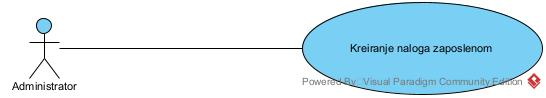
\includegraphics[scale=0.5]{Korisnici/Administrator/UML/SlucajUpotrebe_KreiranjeNalogaZaposlenom.jpg}
    \end{center}
\caption{Dijagram kreiranja naloga zaposlenom.}
\end{figure}

\subsubsection{Slučaj upotrebe: Deaktiviranje naloga osobama koje su prekinule radni odnos}
\begin{enumerate}
    \item \textbf{Kratak opis:} Administrator deaktivira nalog osobi koja prekida radni odnos u kompaniji, pomenuta osoba gubi mogućnost pristupa sistemu.
    \item \textbf{Učesnici:}
        \begin{itemize}
            \item Administrator
        \end{itemize}
    \item \textbf{Preduslovi:} Sistem je u funkciji. Administrator ima pristup internetu, sistemu, kao i privilegije potrebne za deaktiviranje naloga.
    \item \textbf{Postuslovi:} Korisnički nalog je deaktiviran. Korišćenjem korisničkog imena i lozinke nije moguće pristupiti sistemu
    \item \textbf{Osnovni tok:}
        \begin{enumerate}
            \item Administrator otvara stranicu sa listom svih zaposlenih u kompaniji.
            \item Sistem prikazuje listu svih zaposlenih i polje za pretragu zaposlenih po korisničkom imenu
            \item Administrator unosi korisničko ime zaposlenog u polje za pretragu.
            \item Sistem otvara stranicu zaposlenog sa svim pratećim podacima o istom.
            \item Administrator bira deaktivaciju naloga
            \item Sistem otvara stranicu potvrde o zatraženoj akciji uz upozorenje o posledicama operacije
            \item Administrator potvrđuje unos.
        \end{enumerate}
    \item \textbf{Alternativni tokovi:}
        \begin{enumerate}
            \item \textbf{Uneto korisničko ime ne odgovara nijednom zaposlenom.} Ukoliko pretraga zaposlenog po korisničkom imenu ne vrati rezultate, interfejs obaveštava administratora i vraća ga na korak (b).
        \end{enumerate}
    \item \textbf{Podtokovi:} /
    \item \textbf{Specijalni zahtevi:} /
    \item \textbf{Dodatne informacije:} Deaktivacija implicira odloženo brisanje naloga. Nakon deaktivacije nije moguće pristupiti datom nalogu, ali će sam nalog biti zadržan u bazi zaposlenih kroz kraći vremenski period radi lakšeg povraćaja naloga u ekstremnim situacijama (Na primer, u slučaju da je došlo do pogrešnog brisanja naloga). Nalog će biti permanentno obrisan kada pomenuti vremenski period istekne.
\end{enumerate}

\begin{figure} [!ht]
    \begin{center}
        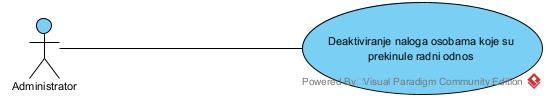
\includegraphics[scale=0.5]{Korisnici/Administrator/UML/SlucajUpotrebe_DeaktiviranjeNaloga.jpg}
    \end{center}
\caption{Dijagram deaktiviranja naloga zaposlenom.}
\end{figure}

\subsubsection{Slučaj upotrebe: Omogućavanje ponovnog pristupa nalogu zaposlenom}
\begin{enumerate}
    \item \textbf{Kratak opis:} Administrator omogućava ponovni pristup nalogu zaposlenom koji sa trenutnim kredencijalima ne može da pristupi sistemu. Gubitak pristupa, kao posledica zaključavanja naloga, može da se desi ukoliko zaposleni pogreši lozinku više od 3 uzastopna puta ili ukoliko nije promenio privremeno generisanu lozinku od strane administratora u predviđenom vremenskom periodu.
    \item \textbf{Učesnici:}
        \begin{itemize}
            \item Administrator
            \item Zaposleni
        \end{itemize}
    \item \textbf{Preduslovi:} Sistem je u funkciji. Administrator ima pristup internetu, sistemu, kao i privilegije potrebne za promenu lozinke zaposlenom.
    \item \textbf{Postuslovi:} Zaposleni uspešno može da pristupi sistemu koristeći novi set kredencijala.
    \item \textbf{Osnovni tok:}
        \begin{enumerate}
            \item Administrator otvara stranicu sa listom svih zaposlenih u kompaniji.
            \item Sistem prikazuje listu svih zaposlenih i polje za pretragu zaposlenih po korisničkom imenu.
            \item Administrator unosi korisničko ime zaposlenog u polje za pretragu.
            \item Sistem otvara stranicu zaposlenog sa svim pratećim podacima o istom.
            \item Administrator bira opciju za uređivanje podataka o zaposlenom.
            \item Administrator generiše novu lozinku za zaposlenog.
            \item Sistem otvara stranicu potvrde o zatraženoj akciji uz upozorenje o posledicama operacije
            \item Administrator potvrđuje unos.
            \item Sistem obaveštava zaposlenog o izvršenoj operaciji putem e-mail adrese zaposlenog, sa novom privremenom lozinkom
        \end{enumerate}
    \item \textbf{Alternativni tokovi:}
        \begin{enumerate}
            \item \textbf{Uneto korisničko ime ne odgovara nijednom zaposlenom.} Ukoliko pretraga zaposlenog po korisničkom imenu ne vrati rezultate, interfejs obaveštava administratora i vraća ga na korak (b).
            \item \textbf{Uneta lozinka odgovara jednoj od prethodnih 10 lozinka za korisnički nalog zaposlenog.} Kako poslednjih 10 lozinki mora biti unikatno, sistem vraća administratora na korak (f)
        \end{enumerate}
    \item \textbf{Podtokovi:} /
    \item \textbf{Specijalni zahtevi:}
        \begin{itemize}
            \item Lozinka mora biti kreirana sa kratkim vremenskim periodom validnosti (na primer 2 dana). Zaposleni mora biti obavešten o datom vremenskom periodu, i ručno promeniti lozinku nakon uspešnog prijavljivanja u sistem.
        \end{itemize}
    \item \textbf{Dodatne informacije:} Administrator ima pristup listi svih zaposlenih u kompaniji.
\end{enumerate}

\begin{figure} [!ht]
    \begin{center}
        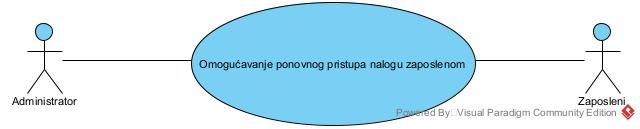
\includegraphics[scale=0.5]{Korisnici/Administrator/UML/SlucajUpotrebe_PonovniPristupNalogu.jpg}
    \end{center}
\caption{Dijagram ponovnog pristupa nalogu zaposlenom.}
\end{figure}

\subsubsection{Slučaj upotrebe: Obezbeđivanje radne opreme zaposlenom}
\begin{enumerate}
    \item \textbf{Kratak opis:} Proces naručivanja i dostave opreme koja je neophodna zaposlenom za svakodnevni rad u kompaniji.
    \item \textbf{Učesnici:}
        \begin{itemize}
            \item Administrator
            \item Zaposleni
        \end{itemize}
    \item \textbf{Preduslovi:} Sistem je u funkciji. Administrator ima pristup internetu, sistemu. Lista opreme neophodna za rad zaposlenog je dostavljena administratoru.
    \item \textbf{Postuslovi:} Oprema je dostavljena administratoru. Zaposleni je obavešten da može da preuzme opremu.
    \item \textbf{Osnovni tok:}
        \begin{enumerate}
            \item Administrator otvara stranicu za naručivanje poslovne opreme.
            \item Sistem prikazuje listu opreme koju je moguće naručiti.
            \item Administrator selektuje opremu koja je neophodna zaposlenom.
            \item Administrator upisuje opravdanje za naručivanje selektovane opreme.
            \item Administrator ponavlja korake (c) i (d) dok sva neophodna oprema nije izabrana i naručivanje opravdano.
            \item Administrator unosi e-mail zaposlenog kome je oprema namenjena.
            \item Administrator bira lokaciju kompanije za dostavljanje preko opadajuće liste lokacija.
            \item Sistem otvara stranicu potvrde o zatraženoj akciji.
            \item Administrator potvrđuje unos.
            \item Sistem čuva informacije o narudžbini.
            \item Administrator može pokrenuti podtok \textbf{(a)} u momentu kada je oprema dostavljena administratoru.
        \end{enumerate}
    \item \textbf{Alternativni tokovi:} /
    \item \textbf{Podtokovi:}
        \begin{enumerate}
            \item \textbf{Obaveštavanje zaposlenog o dostavljenoj opremi:}
                \begin{enumerate}
                    \item Administrator otvara stranicu sa informacijama o narudžbini.
                    \item Administrator potvrđuje da je roba fizički dostavljena na izabranu lokaciju kompanije.
                    \item Administrator potvrđuje da je roba u korektnom stanju.
                    \item Administrator potvrđuje prethodni unos klikom na dugme Završi Narudžbinu.
                    \item Sistem šalje automatsku e-mail poruku zaposlenom da je robu moguće preuzeti.
                    \item Sistem arhivira stranicu o narudžbini.
                \end{enumerate}
        \end{enumerate}
    \item \textbf{Specijalni zahtevi:} /
    \item \textbf{Dodatne informacije:} Obavezna polja za administratora su: e-mail adresa zaposlenog, lokacija dostave, barem jedan komad bilo koje opreme selektovan.
\end{enumerate}

\begin{figure} [!ht]
    \begin{center}
        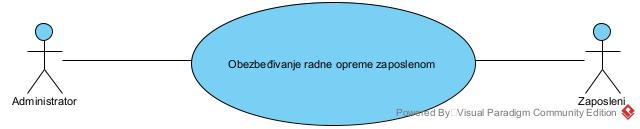
\includegraphics[scale=0.5]{Korisnici/Administrator/UML/SlucajUpotrebe_RadnaOprema.jpg}
    \end{center}
\caption{Dijagram obezbeđivanja radne opreme zaposlenom.}
\end{figure}

\newpage
\subsection{Aktivnosti Menadžera Ljudskih Resursa}

\begin{figure} [!ht]
    \begin{center}
        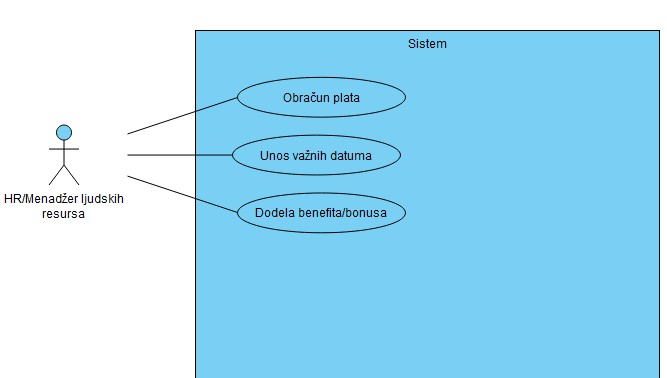
\includegraphics[scale=0.5]{{Korisnici/HR Menadzer ljudskih resursa/UML/hr_use_case_jpg.jpg}}
    \end{center}
\caption{Slučajevi upotrebe Menadžera ljudskih resursa.}
\end{figure}

\subsubsection{Slučaj upotrebe: Unos važnih datuma}
\begin{enumerate}
    \item \textbf{Kratak opis:} HR menadžer vrši unos važnih datuma vezanih za zaposlene, kao što su datumi zapošljavanja, itd.
    \item \textbf{Učesnici:}
        \begin{itemize}
            \item HR menadžer
        \end{itemize}
    \item \textbf{Preduslovi:} HR menadžer je registrovan korisnik sistema. HR menadžer ima pristup podacima o radnicima. Sistem je u funkciji.
    \item \textbf{Postuslovi:} Informacije o važnim datumima su ažurirane u sistemu.
    \item \textbf{Osnovni tok:}
        \begin{enumerate}
            \item HR menadžer otvara stranicu za unos važnih datuma.
            \item Sistem prikazuje listu zaposlenih.
            \item HR menadžer bira zaposlenog za koga želi da unese važan datum.
            \item Sistem prikazuje obrazac za unos datuma.
            \item HR menadžer unosi datum i opis događaja.
            \item HR menadžer pritiskom na dugme potvrđuje unos.
            \item Sistem čuva uneti datum.
            \item Sistem obaveštava HR menadžera o uspešnom unosu važnog datuma.
        \end{enumerate}
    \item \textbf{Alternativni tokovi:} /
    \item \textbf{Podtokovi:} /
    \item \textbf{Specijalni zahtevi:} /
    \item \textbf{Dodatne informacije:} Važni datumi mogu obuhvatati godišnjice zapošljavanja, rođendane, slave itd.
\end{enumerate}

\begin{figure} [!ht]
    \begin{center}
        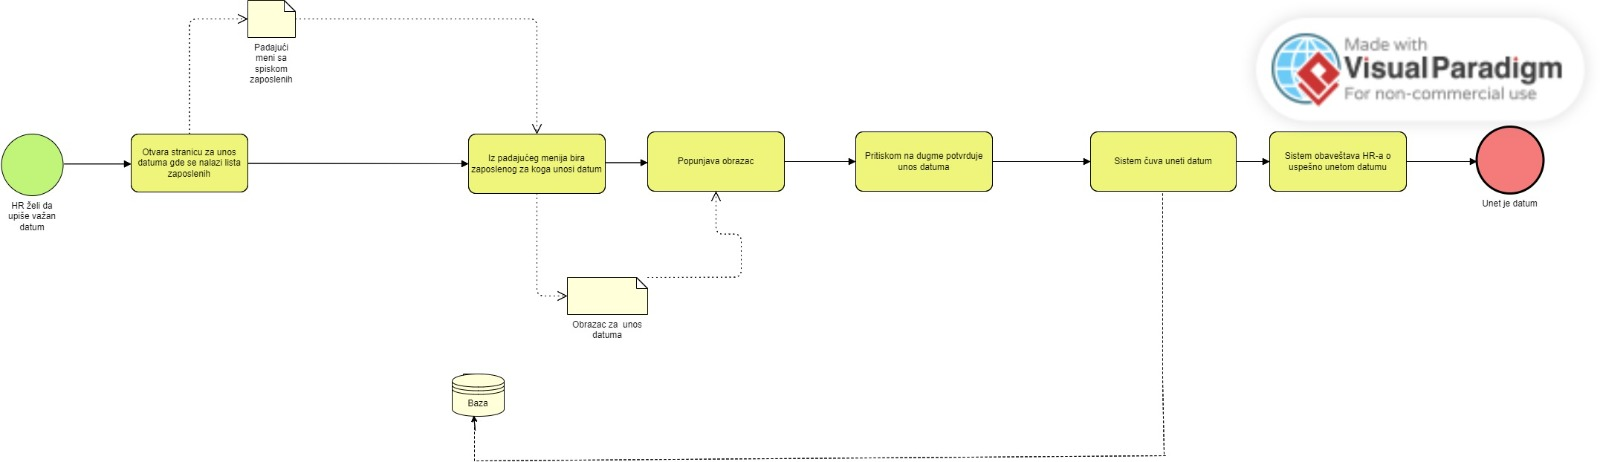
\includegraphics[width=\textwidth,height=\textheight,keepaspectratio]{{Korisnici/HR Menadzer ljudskih resursa/BPMN/upis_datuma.jpg}}
    \end{center}
\caption{Dijagram upisa važnih datuma.}
\end{figure}

\subsubsection{Slučaj upotrebe: Dodela benefita/bonusa}
\begin{enumerate}
    \item \textbf{Kratak opis:} HR menadžer vrši dodelu benefita ili bonusa zaposlenima na osnovu njihovih postignuća ili jubileja  .
    \item \textbf{Učesnici:}
        \begin{itemize}
            \item HR menadžer
        \end{itemize}
    \item \textbf{Preduslovi:} HR menadžer je registrovan korisnik sistema. HR menadžer ima pristup podacima o radnicima. Sistem je u funkciji.
    \item \textbf{Postuslovi:} Informacije o dodeljenim benefitima/bonusima su ažurirane u sistemu.
    \item \textbf{Osnovni tok:}
        \begin{enumerate}
            \item HR menadžer otvara stranicu za dodelu benefita/bonusa.
            \item Sistem prikazuje listu zaposlenih.
            \item HR menadžer bira zaposlenog kome želi dodeliti benefit ili bonus.
            \item Sistem prikazuje obrazac za unos informacija o dodeli benefita/bonusa.
            \item HR menadžer unosi vrstu benefita/bonusa, iznos ili opis.
            \item HR menadžer pritiskom na dugme potvrđuje dodelu.
            \item Sistem čuva informacije o dodeljenom benefitu/bonusu.
            \item Sistem obaveštava HR menadžera o uspešnoj dodeli benefita/bonusa.
        \end{enumerate}
    \item \textbf{Alternativni tokovi:}
        \begin{enumerate}
            \item \textbf{HR menadžer nije uneo potrebne informacije.} Ako HR menadžer u koraku (e) nije uneo vrstu benefita/bonusa, iznos ili opis, sistem obaveštava HR menadžera i vraća ga na korak (d).
        \end{enumerate}
    \item \textbf{Podtokovi:} /
    \item \textbf{Specijalni zahtevi:}
        \begin{itemize}
            \item Zahteva se obavezno polje za unos vrste benefita/bonusa.
            \item Opciono je polje za unos iznosa ili dodatnih opisa.
        \end{itemize}
    \item \textbf{Dodatne informacije:} Dodela benefita može obuhvatiti dodatke na platu, dodatne slobodne dane, poklone itd.
\end{enumerate}

\begin{figure} [!ht]
    \begin{center}
        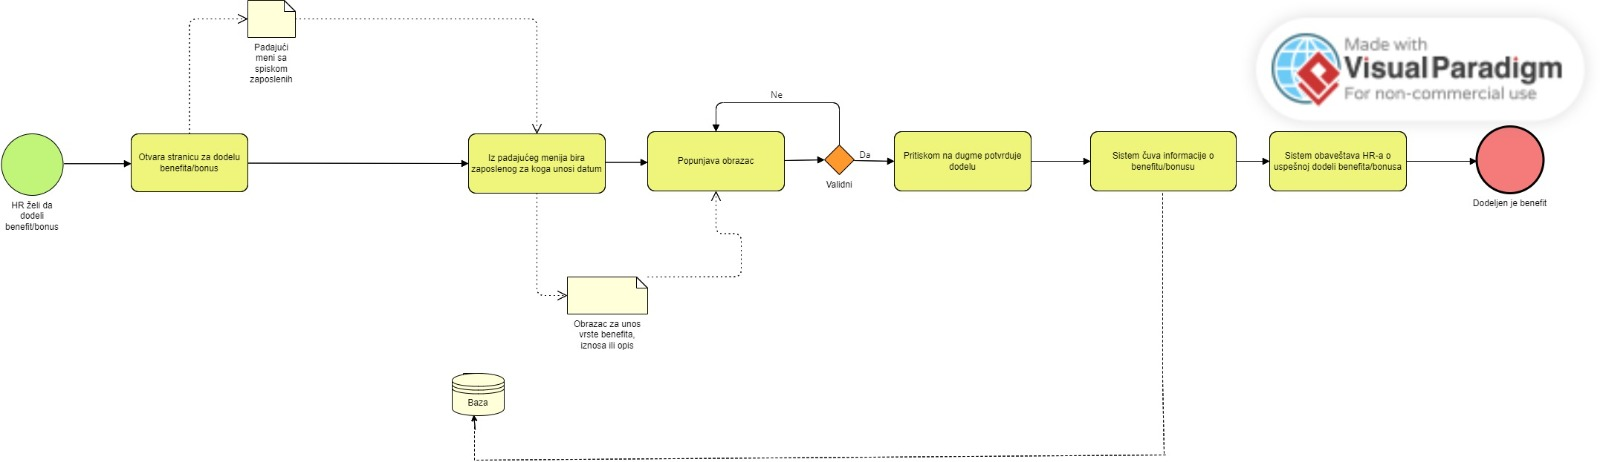
\includegraphics[width=\textwidth,height=\textheight,keepaspectratio]{{Korisnici/HR Menadzer ljudskih resursa/BPMN/dodela_benefita.jpg}}
    \end{center}
\caption{Dijagram dodele benefita zaposlenima.}
\end{figure}

\subsubsection{Slučaj upotrebe: Obračun plata}
\begin{enumerate}
    \item \textbf{Kratak opis:} HR menadžer vrši obračun plata za zaposlene u firmi.
    \item \textbf{Učesnici:}
        \begin{itemize}
            \item HR menadžer
        \end{itemize}
    \item \textbf{Preduslovi:} HR menadžer je registrovan korisnik sistema. HR menadžer ima pristup podacima o radnicima i njihovim platama. Sistem je u funkciji.
    \item \textbf{Postuslovi:} Obračun plata je izvršen, i informacije o platama su ažurirane u sistemu.
    \item \textbf{Osnovni tok:}
        \begin{enumerate}
            \item HR menadžer otvara stranicu za obračun plata.
            \item Sistem prikazuje listu zaposlenih.
            \item HR menadžer bira zaposlenog za koga želi da izvrši obračun plate.
            \item Sistem prikazuje podatke o radniku, uključujući radne sate, dodatke, odbitke itd.
            \item HR menadžer unosi ili proverava podatke, vrši i potvrđuje obračun plate.
            \item Sistem čuva izmene u platama.
            \item Sistem obaveštava HR menadžera o uspešnom obračunu plata.
        \end{enumerate}
    \item \textbf{Alternativni tokovi:}
        \begin{enumerate}
            \item \textbf{HR menadžer nije uneo potrebne informacije.} Ako HR menadžer u koraku (e) nije uneo sve potrebne informacije (npr. radne sate), sistem obaveštava HR menadžera i vraća ga na korak (d).
        \end{enumerate}
    \item \textbf{Podtokovi:} /
    \item \textbf{Specijalni zahtevi:} /
    \item \textbf{Dodatne informacije:} HR menadžer može pregledati istoriju obračuna plata za svakog zaposlenog.
\end{enumerate}

\newpage
\subsection{Aktivnosti Vodje Tima}

\begin{figure} [!ht]
    \begin{center}
        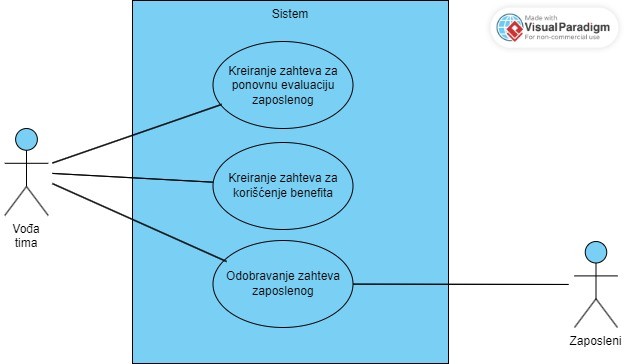
\includegraphics[scale=0.5]{{Korisnici/Vodja tima/UML/team_lead_use_case.jpg}}
    \end{center}
\caption{Slučajevi upotrebe Vodje Tima.}
\end{figure}

\subsubsection{Slučaj upotrebe: Kreiranje zahteva za ponovnu evaluaciju zaposlenog}
\begin{enumerate}
    \item \textbf{Kratak opis:} Nakon što vođa tima proceni da je na osnovu rada zaposlenog potrebno ponovo odraditi evaluaciju njegovog rada, kako bi utvrdili da li radnik zaslužuje povećanje senioriteta, vođa tima kreira zahtev za evaluaciju koji sistem čuva.
    \item \textbf{Učesnici:}
        \begin{itemize}
            \item Vođa tima
        \end{itemize}
    \item \textbf{Preduslovi:} Vođa tima je registrovan korisnik sistema. Vođa tima ima pristup internetu. Sistem je u funkciji.
    \item \textbf{Postuslovi:} Zahtev za evaluaciju je sačuvan u sistemu. Baza je ažurirana.
    \item \textbf{Osnovni tok:}
        \begin{enumerate}
            \item Vođa tima otvara stranicu gde se nalazi dugme za kreiranje zahteva za evaluaciju.
            \item Vođa tima pritiska dugme za kreiranje zahteva za evaluaciju.
            \item Sistem mu prikazuje obrazac za kreiranje novog zahteva i padajući meni za izbor zaposlenog za koga se kreira zahtev.
            \item Vođa tima iz padajućeg menija bira zaposlenog za koga kreira zahtev za evaluaciju.
            \item Vođa tima popunjava popunjava obrazac.
            \item Vođa tima pritiskom na dugme potvrđuje kreiranje novog zahteva.
            \item Sistem vrši validaciju unetih podataka.
            \item Sistem čuva kreirani zahtev za evaluaciju.
            \item Sistem obaveštava vođu tima o uspešno kreiranom zahtevu.
        \end{enumerate}
    \item \textbf{Alternativni tokovi:}
        \begin{enumerate}
            \item \textbf{Vođa tima je uneo nevalidne podatke}. Ukoliko u koraku (g) sistem utvrdi da je vođa tima ostaio neko obavezno polje prazno ili da vođa tima nije izabrao nijednog zaposlenog, sistem obaveštava vođu tima obeležavanjem neispravnog polja. Proces se nastavlja u koraku (d).
        \end{enumerate}
    \item \textbf{Podtokovi:} /
    \item \textbf{Specijalni zahtevi:} /
    \item \textbf{Dodatne informacije:} Potrebni podaci za popunjavanje obrazca su: obrazloženje zašto se kreira novi zahtev za evaluaciju zaposlenog.
\end{enumerate}

\begin{figure} [!ht]
    \begin{center}
        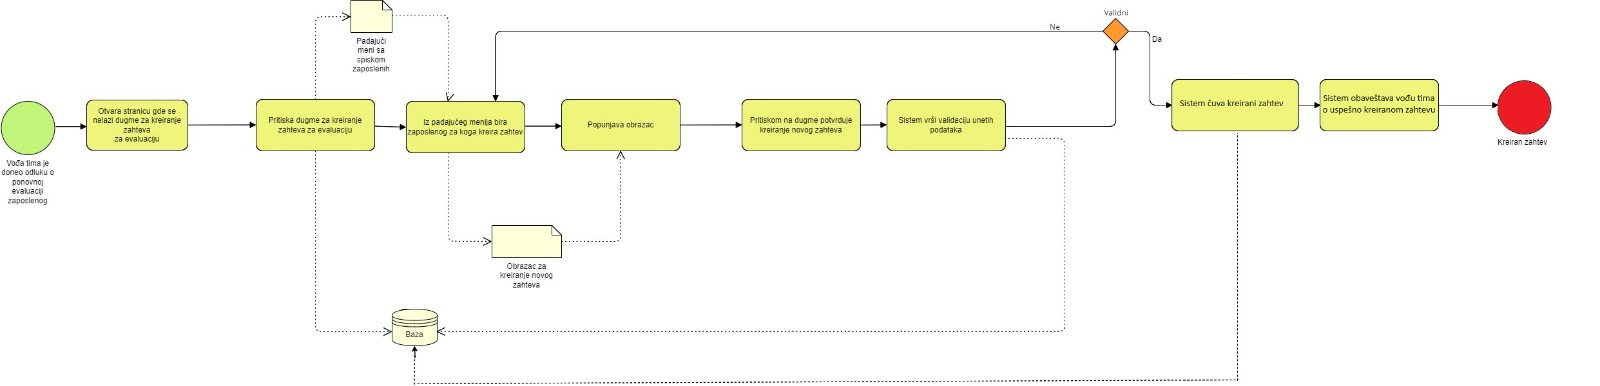
\includegraphics[width=\textwidth,height=\textheight,keepaspectratio]{{Korisnici/Vodja tima/BPMN/kreiranje_zahteva_za_ponovnu_evaluaciju_zaposlenog.jpeg}}
    \end{center}
\caption{Dijagram zahteva za ponovnu evaluaciju zaposlenog.}
\end{figure}

\subsubsection{Slučaj upotrebe: Kreiranje zahteva za korišćenje benefita}
\begin{enumerate}
    \item \textbf{Kratak opis:} Nakon što vođa tima odluči da određeni zaposleni treba da iskoristi benefit koji firma pruža, vođa tima kreira zahtev za korišćenje benefita od strane zaposlenog.
    \item \textbf{Učesnici:}
        \begin{itemize}
            \item Vođa tima
        \end{itemize}
    \item \textbf{Preduslovi:} Vođa tima je registrovan korisnik sistema. Vođa tima ima pristup internetu. Sistem je u funkciji.
    \item \textbf{Postuslovi:} Zahtev za korišćenje benefita je sačuvan u sistemu. Baza je ažurirana.
    \item \textbf{Osnovni tok:}
        \begin{enumerate}
            \item Vođa tima otvara stranicu gde se nalazi dugme za kreiranje zahteva za korišćenje benefita.
            \item Vođa tima pritiska dugme za kreiranje zahteva za korišćenje benefita.
            \item Sistem mu prikazuje obrazac za kreiranje novog zahteva i padajući meni za izbor zaposlenog za koga se kreira zahtev.
            \item Vođa tima iz padajućeg menija bira zaposlenog za koga kreira zahtev.
            \item Vođa tima iz padajućeg menija bira vrstu benefita.
            \item Vođa tima popunjava obrazac.
            \item Vođa tima pritiskom na dugme potvrđuje kreiranje novog zahteva.
            \item Sistem vrši validaciju unetih podataka.
            \item Sistem čuva kreirani zahtev.
            \item Sistem obaveštava vođu tima o uspešno kreiranom zahtevu.
        \end{enumerate}
    \item \textbf{Alternativni tokovi:}
        \begin{enumerate}
            \item \textbf{Vođa tima je uneo nevalidne podatke}. Ukoliko u koraku (g) sistem utvrdi da je vođa tima ostaio neko obavezno polje prazno ili da vođa tima nije izabrao nijednog zaposlenog, sistem obaveštava vođu tima obeležavanjem neispravnog polja. Proces se nastavlja u koraku (d).
        \end{enumerate}
    \item \textbf{Podtokovi:} /
    \item \textbf{Specijalni zahtevi:} /
    \item \textbf{Dodatne informacije:} Potrebni podaci za popunjavanje obrazca su: Tip benefita koji zaposleni treba da iskoristi, obrazloženje zašto je potrebno da ga iskoristi, opis kako će benefit uticati na njegov rad i cena koju bi firma trebalo da plati.
\end{enumerate}

\begin{figure} [!ht]
    \begin{center}
        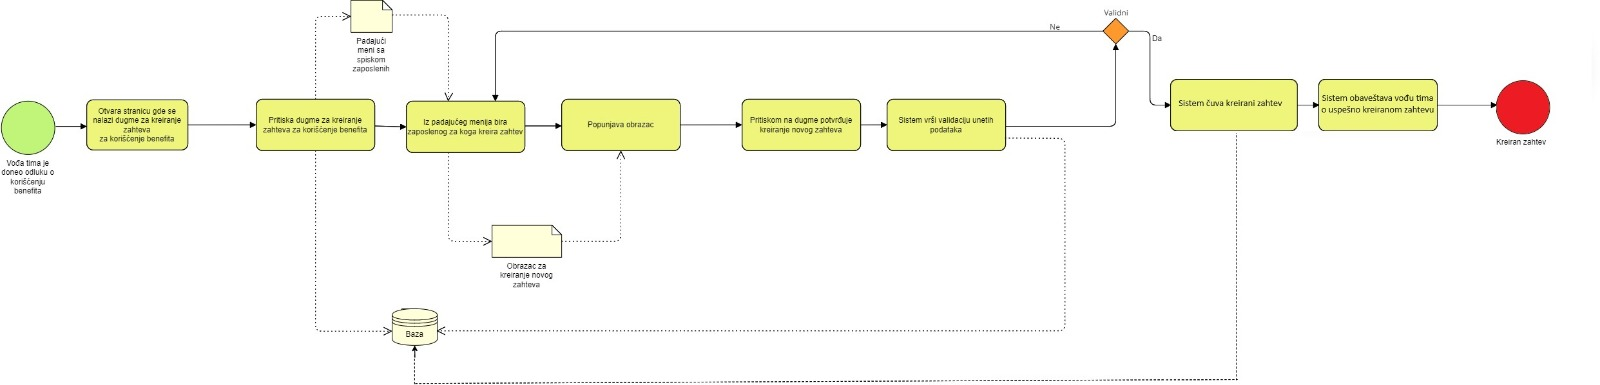
\includegraphics[width=\textwidth,height=\textheight,keepaspectratio]{{Korisnici/Vodja tima/BPMN/kreiranje_zahteva_za_koriscenje_benefita.jpeg}}
    \end{center}
\caption{Dijagram zahteva za korišćenje benefita.}
\end{figure}

\subsubsection{Slučaj upotrebe: Odobravanje zahteva zaposlenog}
\begin{enumerate}
    \item \textbf{Kratak opis}: Na osnovu obrazloženog zahteva koji je zaposleni kreirao, vođa tima odobrava zahtev. Sistem beleži promenu statusa zahteva zaposlenog.
    \item \textbf{Učesnici:}
        \begin{itemize}
            \item Vođa tima
            \item Zaposleni
        \end{itemize}
    \item \textbf{Preduslovi:} Vođa tima je registrovan korisnik sistema. Vođa tima ima pristup internetu. Sistem je u funkciji. Postoji zahtev od bar jednog zaposlenog.
    \item \textbf{Postuslovi:} Ažuriran je zahtev koji je kreirao zaposleni. Baza je ažurirana.
    \item \textbf{Osnovni tok:}
        \begin{enumerate}
            \item Vođa tima otvara stranicu sa svim zahtevima zaposlenih iz njegovog tima.
            \item Vođa tima pritiska dugme za otvaranje informacija o konkretnom zahtevu.
            \item Sistem mu prikazuje informacije o zahtevu i padajući meni sa opcijama potvrdi ili odbij.
            \item Vođa tima bira opciju iz padajućeg menija.
            \item Vođa tima pritiskom na dugme potvrđuje promene.
            \item Sistem čuva promenu statusa zahteva.
            \item Sistem obaveštava vođu tima o uspešnoj promeni statusa.
        \end{enumerate}
    \item \textbf{Alternativni tokovi:}
        \begin{enumerate}
            \item \textbf{Vođa tima nije izabrao opciju potvrdi.} Ako vođa tima u koraku (e) nije izabrao jednu od dve opcije iz padajućeg menija ili je izabrao odbij, sistem neće evidentirati promenu statusa. Proces se nastavlja iz koraka (b).
        \end{enumerate}
    \item \textbf{Podtokovi:} /
    \item \textbf{Specijalni zahtevi:} Mora postojati obrazloženje od strane zaposlenog u zahtevu, zašto je zahtev kreiran.
    \item \textbf{Dodatne informacije:} Zahtevi zaposlenog mogu biti zahtev za rad od kuće i zahtev za korišćenje benefita.
\end{enumerate}

\begin{figure} [!ht]
    \begin{center}
        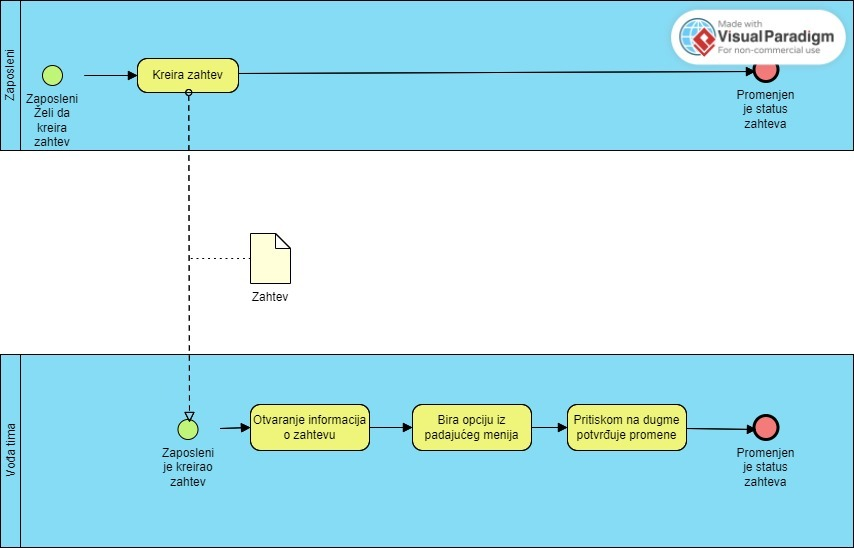
\includegraphics[width=\textwidth,height=\textheight,keepaspectratio]{{Korisnici/Vodja tima/BPMN/Dijagram_saradnje_odobravanje_zahteva_zaposlenog.jpeg}}
    \end{center}
\caption{Dijagram za odobravanje zahteva zaposlenog.}
\end{figure}

\newpage
\subsection{Aktivnosti Zaposlenog}

\subsubsection{Slučaj upotrebe: Pregled dana i unetih radnih sati za odredjeni mesec}
\begin{enumerate}
    \item \textbf{Kratak opis:} Zaposleni na osnovu odabira meseca pregleda radne dane, unete sate i kratke opise poslova.
    \item \textbf{Učesnici:}
        \begin{itemize}
            \item Zaposleni
        \end{itemize}
    \item \textbf{Preduslovi:} Zaposleni je registrovani korisnik sistema.
    \item \textbf{Postuslovi:} Zaposlenom je prikazana lista tiketa za odabrani mesec, gde je za svaki tiket prikazan dan, broj sati odrađenih za taj dan i kratak opis posla odrađenog za taj dan.
    \item \textbf{Osnovni tok:}
        \begin{enumerate}
            \item Zaposleni otvara stranicu za unošenje radnih sati.
            \item U padajućoj listi zaposleni bira za koji mesec želi da mu se prikažu uneti dani sa odgovarajućim podacima.
            \item Sistem vrši obradu zahteva.
            \item Na stranici se prikazuje lista tiketa, gde svaki tiket sadrži podatke o unetom danu, broju radnih sati za taj dan i opisu odradjenog posla.
        \end{enumerate}
    \item \textbf{Alternativni tokovi:} 
        \begin{enumerate}
            \item \textbf{Zaposleni je odabrao tekući mesec u padajućoj listi}. Ukoliko u koraku (b) zaposleni odabere tekući mesec, zaposlenom se nakon završetka procesa (d) prikazuje dugme sa opcijom dodavanja novog tiketa.
        \end{enumerate}
    \item \textbf{Podtokovi:} /
    \item \textbf{Specijalni zahtevi:} /
    \item \textbf{Dodatne informacije:} /
\end{enumerate}

\subsubsection{Slučaj upotrebe: Unošenje radnih sati}
\begin{enumerate}
    \item \textbf{Kratak opis:} Zaposleni unosi broj odrađenih ranih sati za konkretan dan kao i opis odrađenog posla.
    \item \textbf{Učesnici:}
        \begin{itemize}
            \item Zaposleni
        \end{itemize}
    \item \textbf{Preduslovi:} Zaposleni je registrovani korisnik sistema i na stranici za pregled radnih sati je odabrao tekući mesec.
    \item \textbf{Postuslovi:} Odrađen broj radnih sati za konkretan dan je sačuvan u sistemu. Baza je ažurirana. Na stranici se prikazuje novi tiket koji je u nerazrešenom statusu.
    \item \textbf{Osnovni tok:}
        \begin{enumerate}
            \item Zaposleni pritiska dugme za dodavanje novog tiketa.
            \item Prikazuje se forma koji sadrži polja za odabir dana, broj odrađenih radnih sati, i opis odrađenog posla.
            \item Zaposleni popunjava formu.
            \item Potvrđuje unos za taj dan.
            \item Sistem vrši obradu podataka.
            \item Sistem čuva unete podatke u bazi podataka.
            \item Na stranici se dodaje tiket koji je u nerazrešenom statusu i informacije koje je korisnik uneo za taj dan.
        \end{enumerate}
    \item \textbf{Alternativni tokovi:}
        \begin{enumerate}
            \item \textbf{Zaposleni je odabrao nevalidan dan}. Ukoliko u koraku (d) korisnik potvrdi unos za dan za koji je uneo radne sate ili dan koji je ispred trenutnog dana ili unese negativan broj za radne sate, prikazuje mu se odgovarajuća poruka o grešci. Proces se nastavlja u koraku (c).
        \end{enumerate}
    \item \textbf{Podtokovi:} /
    \item \textbf{Specijalni zahtevi:} /
    \item \textbf{Dodatne informacije:} Polje za unošenje broja radnih sati je obavezno.
\end{enumerate}

\begin{figure} [!ht]
    \begin{center}
        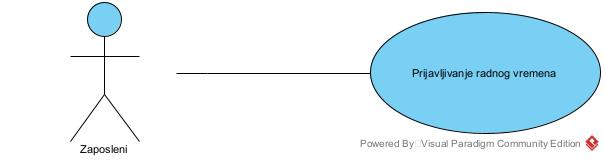
\includegraphics[scale=0.5]{Korisnici/Zaposleni/UML/PrijavljivanjeRadnogVremena.jpg}
    \end{center}
\caption{Dijagram prijavljivanja radnog vremena.}
\end{figure}

\subsubsection{Slučaj upotrebe: Izmena tiketa}
\begin{enumerate}
    \item \textbf{Kratak opis:} Zaposleni menja informacije u tiketu za konkretan dan.
    \item \textbf{Učesnici:}
        \begin{itemize}
            \item Zaposleni
        \end{itemize}
    \item \textbf{Preduslovi:} Zaposleni je registrovani korisnik sistema, na stranici za pregled radnih sati je odabrao tekući mesec i tiket za dan čije informacije korisnik želi da menja je prikazan na stranici, postoji u sistemu i u nerazrešenom je statusu.
    \item \textbf{Postuslovi:} Informacije su ažurirane u sistemu i korisnik vidi promene na tiketu .
    \item \textbf{Osnovni tok:}
        \begin{enumerate}
            \item Zaposleni pritiska odgovarajuće dugme za izmenu podataka na tiketu.
            \item Na tiketu polja za unošenje radnih sati i opis odrađenog posla postaju moguća za izmenu.
            \item Zaposleni menja odgovarajuća polja.
            \item Potvrđuje izmene.
            \item Sistem vrši obradu podataka.
            \item Sistem čuva unete podatke u bazi podataka.
            \item Na stranici se prikazuje tiket u izmenjenom obliku.
        \end{enumerate}
    \item \textbf{Alternativni tokovi:}
        \begin{enumerate}
            \item \textbf{Zaposleni je odabrao nevalidan broj radnih sati}. Ukoliko u koraku (c) zaposleni unese radne sate koji predstavljaju negativan broj, prikazuje mu se odgovarajuća poruka o grešci. Proces se nastavlja u koraku (c).
        \end{enumerate}
    \item \textbf{Podtokovi:} /
    \item \textbf{Specijalni zahtevi:} /
    \item \textbf{Dodatne informacije:} Polje za unosenje broja radnih sati je obavezno.
\end{enumerate}

\begin{figure} [!ht]
    \begin{center}
        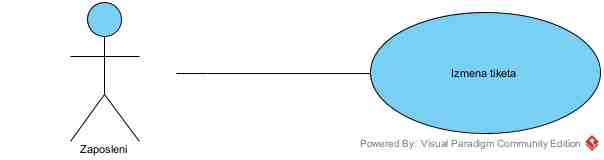
\includegraphics[width=\textwidth,height=\textheight,keepaspectratio]{Korisnici/Zaposleni/UML/IzmenaTiketa.jpg}
    \end{center}
\caption{Dijagram izmene tiketa.}
\end{figure}

\subsubsection{Slučaj upotrebe: Kreiranje zahteva}
\begin{enumerate}
    \item \textbf{Kratak opis:} Zaposleni na osnovu unete opcije i popunjavanja odgovarajucih polja kreira zahtev, koji je nakon kreiranja u statusu nerazrešen.
    \item \textbf{Učesnici:}
        \begin{itemize}
            \item Zaposleni
        \end{itemize}
    \item \textbf{Preduslovi:} Zaposleni je registrovan korisnik sistema.
    \item \textbf{Postuslovi:} Zahtev je uspešno kreiran i sačuvan je u sistemu. Baza je ažurirana i na stranici za prikaz zahteva je dodat novokreirani zahtev
    \item \textbf{Osnovni tok:}
        \begin{enumerate}
            \item Zaposleni otvara stranicu za kreiranje zahteva.
            \item U padajućoj listi bira tip zahteva koji želi da kreira.
            \item Ako je odabrana opcija za rad od kuće, izvršava se podtok (a), ako je odabrana opcija za koriscenje benefita izvršava se podtok (b), ako je izabrana opcija za godišnji odmor izvršava se podtok (c), ako je odabrana opcija za sick leave (d), a ako je odabrana opcija za reevaluaciju izvršava se podtok (e).
            \item Nakon popunjavanja forme, pritiska dugme za potvrdu unosa podataka.
            \item Sistem vrši obradu unosa. Baza je ažurirana. Stranica sa zahtevima je ažurirana.
            \item Na stranici se prikazuje poruka o uspešno kreiranom zahtevu.
        \end{enumerate}
    \item \textbf{Podtokovi:}
        \begin{enumerate}
            \item Rad od kuće
            \begin{enumerate}
                \item Na stranici se prikazuje forma koja sadrži polje za unos datuma kao i polje gde se navodi razlog za zahtev za rad od kuće.
                \item Klikom na polje za unos datuma, zaposlenom se prikazuje padajuci prozor za odabir datuma.
                \item Zaposleni odabira datum.
                \item Zaposleni navodi razlog za podnošenje zahteva. 
            \end{enumerate}
            \item Korišćenje benefita
            \begin{enumerate}
                \item Na stranici se prikazuje padajuća lista sa tipom benefita koji zaposleni želi da odabere.
                \item Zaposleni bira tip benefita.
            \end{enumerate}
            \item Godišnji odmor
            \begin{enumerate}
                \item Na stranici se prikazuje forma koja sadrži dva polja za unos datuma, koja predstavljaju period korišćenja godišnjeg odmora.
                \item Zaposleni preko padajućeg menija bira datum početka i datum kraja korišćenja godišnjeg odmora. 
            \end{enumerate}
            \item Sick leave
            \begin{enumerate}
                \item Na stranici se prikazuje forma koja sadrži dva polja za unos datuma koja predstavljaju period korišćenja godišnjeg odmora, kao i dugme za unos lekarskog izveštaja.
                \item Zaposleni preko padajućeg menija bira datum početka i datum kraja korišćenja sick leave-a.
                \item Zaposleni klikom na dugme unosi dokument koji predstavlja lekarski izveštaj.
            \end{enumerate}
            \item Re-evaluacija
            \begin{enumerate}
                \item Na stranici se prikazuje forma koja sadrži polje gde se unosi razlog za evaluaciju.
            \end{enumerate}
    \end{enumerate}
    \item \textbf{Alternativni tokovi:}
            \begin{enumerate}
                \item Ako je u koraku (iii) podtoka (a) odabran dan koji je u prošlom vremenu(iza trenutnog dana) na ekranu će se prikazati odgovarajuća poruka o grešci. Proces se nastavlja u koraku (iii) podtoka (a).
                \item Ako su u koraku (ii) podtoka (c) odabrani dani sa kojima se premašuje broj dana odmora, na ekranu će se prikazati odgovarajuća poruka o grešci. Proces se nastavlja u koraku (ii) podtoka (c).
                \item Ako su u koraku (ii) podtoka (d) odabrani dani sa kojima se premašuje broj sick leave-a, na ekranu će se prikazati odgovarajuća poruka o grešci. Proces se nastavlja u koraku (ii) podtoka (d). 
            \end{enumerate}
    \item \textbf{Specijalni zahtevi:} /
    \item \textbf{Dodatne informacije:} /
\end{enumerate}

\begin{figure} [!ht]
    \begin{center}
        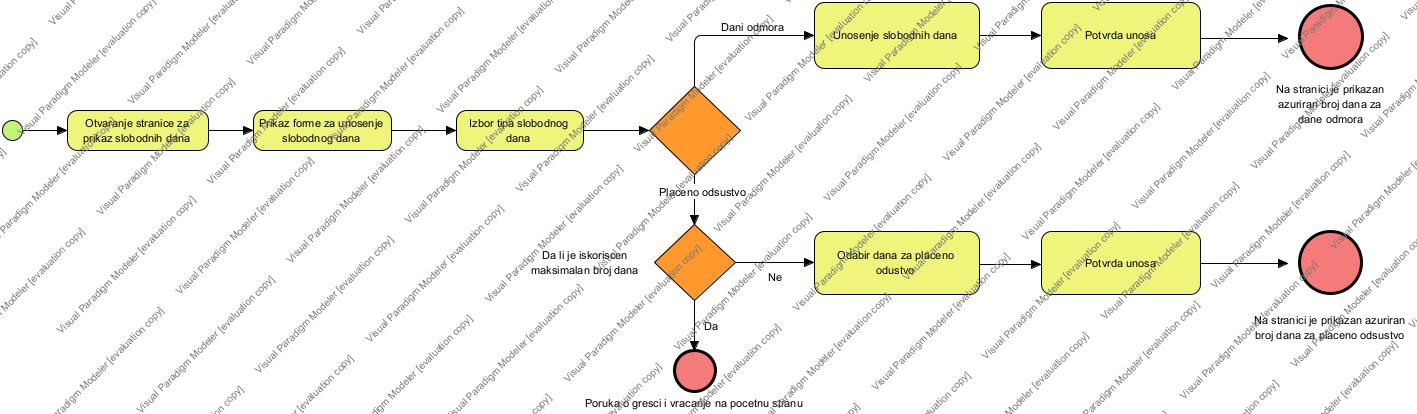
\includegraphics[width=\textwidth,height=\textheight,keepaspectratio]{{Korisnici/Zaposleni/UML/Prijavljivanje slobodnih dana.jpg}}
    \end{center}
\caption{Dijagram prijavljivanja slobodnih dana.}
\end{figure}

\newpage
\subsubsection{Slučaj upotrebe: Pregled iskorišćenosti dana odmora i sick leave-a}
\begin{enumerate}
    \item \textbf{Kratak opis:} Zaposleni na osnovu odabira tipa odsustva(godišnji odmor ili sick leave) pregleda broj neiskorišćenih dana za odabrani tip odsustva.
    \item \textbf{Učesnici:}
        \begin{itemize}
            \item Zaposleni
        \end{itemize}
    \item \textbf{Preduslovi:} Zaposleni je registrovani korisnik sistema.
    \item \textbf{Postuslovi:} Zaposlenom je prikazan broj neiskorišćenih dana za odabrani tip odsustva, kao i lista iskorišćenih dana odsustva.
    \item \textbf{Osnovni tok:}
        \begin{enumerate}
            \item Zaposleni otvara stranicu za pregled odmora.
            \item U padajućoj listi zaposleni bira da li želi da mu se prikaže broj slobodnih dana odmora ili sick leave-a.
            \item Sistem vrši obradu zahteva.
            \item U zavisnosti od odabranog tipa na ekranu se prikazuje o broju preostalih dana za odabrani tip kao i lista iskorišćenih dana.
        \end{enumerate}
    \item \textbf{Alternativni tokovi:} /
    \item \textbf{Podtokovi:} /
    \item \textbf{Specijalni zahtevi:} /
    \item \textbf{Dodatne informacije:} /
\end{enumerate}


\subsubsection{Slučaj upotrebe: Pregled zahteva zaposlenog}
\begin{enumerate}
    \item \textbf{Kratak opis:} Zaposleni na osnovu odabira statusa zahteva(ne razrešen, odobren ili odbijen) pregleda kreirane zahteve od statusa kojeg je odabrao.
    \item \textbf{Učesnici:}
        \begin{itemize}
            \item Zaposleni
        \end{itemize}
    \item \textbf{Preduslovi:} Zaposleni je registrovani korisnik sistema.
    \item \textbf{Postuslovi:} Zaposlenom je prikazana lista zahteva na osnovu statusa kojeg je odabrao.
    \item \textbf{Osnovni tok:}
        \begin{enumerate}
            \item Zaposleni otvara stranicu za pregled zahteva.
            \item U padajućoj listi zaposleni bira status zahteva.
            \item Sistem vrši obradu zahteva.
            \item U zavisnosti od odabranog statusa na ekranu se prikazuje lista zahteva koje je korisnik kreirao.
        \end{enumerate}
    \item \textbf{Alternativni tokovi:} /
    \item \textbf{Podtokovi:} /
    \item \textbf{Specijalni zahtevi:} /
    \item \textbf{Dodatne informacije:} /
\end{enumerate}

\newpage
\subsection{Aktivnosti Udruženja}

\subsubsection{Slučaj upotrebe: Zahtev za osnivanje udruženja}
\begin{enumerate}
    \item \textbf{Kratak opis:} Zaposleni u kompaniji šalje zahtev za osnivanje udruženja.
    \item \textbf{Učesnici:}
        \begin{itemize}
            \item Zaposleni
        \end{itemize}
    \item \textbf{Preduslovi:} Sistem je u funkciji. Zaposleni ima pristup internetu i sistemu.
    \item \textbf{Postuslovi:} Zahtev za osnivanje udruženja je uspešno podnet i u statusu je čekanja za odobravanje. Vlasnik udruženja je obavešten.
    \item \textbf{Osnovni tok:}
        \begin{enumerate}
            \item Zaposleni otvara stranicu za udruženja.
            \item Klikom na dugme za osnivanje novog udruženja prikazuje se forma koja sadrži polje gde se bira tip udruženja.
            \item Za slučaj da je tip udruženja sportska sekcija, izvršava se podtok (a), za programersku sekciju podtok (b), a za ostalo podtok (c).
            \item Zaposleni popunjava formular.
            \item Zaposleni potvrđuje podnošenje zahteva.
            \item Sistem beleži zahtev za osnivanje udruženja i obaveštava Menadžere ljudskih resursa za validaciju.
        \end{enumerate}
    \item \textbf{Podtokovi:}
        \item Sportska sekcija
            \begin{enumerate}
                \item Zaposlenom se prikazuje forma gde se bira sport i polje gde se navode dodatne informacije.
            \end{enumerate}
        \item Programerska sekcija
            \begin{enumerate}
                \item Zaposlenom se prikazuje forma gde se unosi programski jezik za koji želi da osnuje zajednicu i polje gde se navode dodatne informacije.
            \end{enumerate}
        \item Ostalo
            \begin{enumerate}
                \item Zaposlenom se prikazuje forma gde se navodi naziv udruženja koji želi da osnuje, polje gde se navodi opis udruženja i polje gde se navode dodatne informacije.
            \end{enumerate}
    \item \textbf{Alternativni tokovi:}
        \begin{enumerate}
            \item \textbf{Formular nije ispravno popunjen.} Sistem obaveštava zaposlenog o greškama na formularu i vraća ga na korak (e).
        \end{enumerate}
    \item \textbf{Podtokovi:} /
    \item \textbf{Specijalni zahtevi:} /
    \item \textbf{Dodatne informacije:} /
\end{enumerate}

\begin{figure} [!ht]
    \begin{center}
        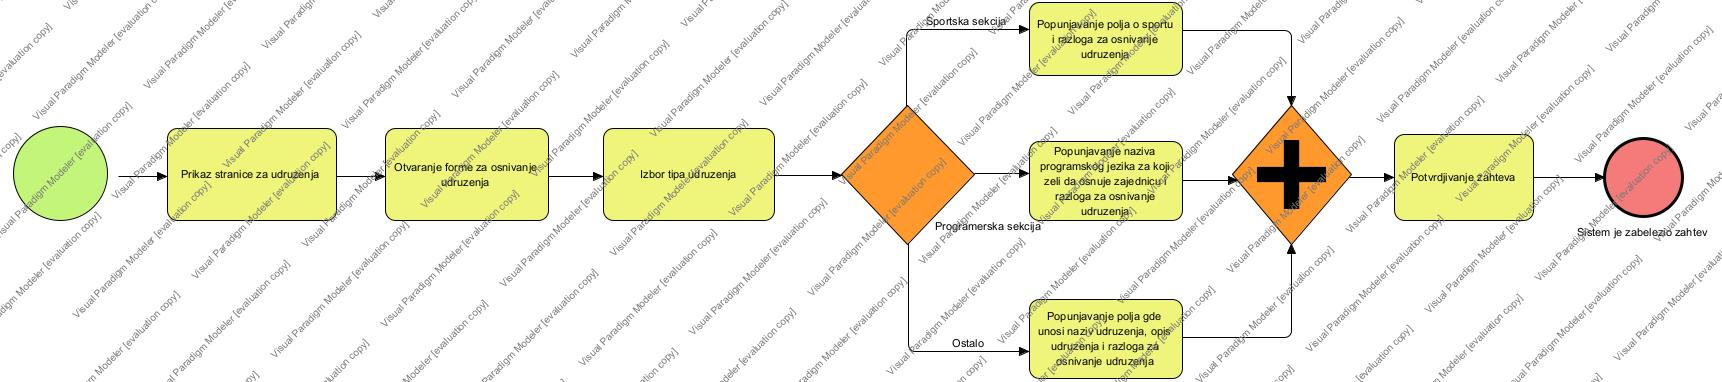
\includegraphics[width=\textwidth,height=\textheight,keepaspectratio]{Korisnici/Udruzenje/BPMN/ZahtevZaOsnivanjeUdruzenja.jpg}
    \end{center}
\caption{Dijagram zahteva za osnivanje udruženja.}
\end{figure}

\subsubsection{Slučaj upotrebe: Zahtev za članstvo u udruženju}
\begin{enumerate}
    \item \textbf{Kratak opis:} Zaposleni u kompaniji šalje zahtev za članstvo u određenom udruženju unutar kompanije.
    \item \textbf{Učesnici:}
        \begin{itemize}
            \item Zaposleni
        \end{itemize}
    \item \textbf{Preduslovi:} Sistem je u funkciji. Zaposleni ima pristup internetu i sistemu.
    \item \textbf{Postuslovi:} Zahtev za članstvo je uspešno podnet. Vlasnik udruženja je obavešten.
    \item \textbf{Osnovni tok:}
        \begin{enumerate}
            \item Zaposleni otvara stranicu za udruženja.
            \item Sistem prikazuje listu svih postojećih udruženja.
            \item Zaposleni otvara stranicu udruženja za koje želi podneti zahtev za članstvo.
            \item Zaposleni otvara stranicu za članstvo u udruženju.
            \item Zaposleni se prijavljuje za članstvo pritiskom na dugme Želim da Postanem Član.
            \item Zaposleni potvrđuje podnošenje zahteva.
            \item Sistem beleži zahtev za članstvo i obaveštava vlasnika udruženja.
        \end{enumerate}
    \item \textbf{Alternativni tokovi:} /
    \item \textbf{Podtokovi:} /
    \item \textbf{Specijalni zahtevi:} /
    \item \textbf{Dodatne informacije:} /
\end{enumerate}

\begin{figure} [!ht]
    \begin{center}
        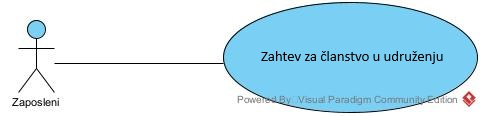
\includegraphics[scale=0.5]{Korisnici/Udruzenje/UML/SlucajUpotrebe_Clanstvo.jpg}
    \end{center}
\caption{Dijagram za članstvo u udruženju.}
\end{figure}

\subsubsection{Slučaj upotrebe: Zahtev za održavanje događaja}
\begin{enumerate}
    \item \textbf{Kratak opis:} Zaposleni koji ima ulogu vlasnika udruženja šalje zahtev za održavanje događaja.
    \item \textbf{Učesnici:}
        \begin{itemize}
            \item Zaposleni
        \end{itemize}
    \item \textbf{Preduslovi:} Sistem je u funkciji. Zaposleni ima pristup internetu i sistemu.
    \item \textbf{Postuslovi:} Zahtev za održavanje događaja je podnet.
    \item \textbf{Osnovni tok:}
        \begin{enumerate}
            \item Zaposleni otvara stranicu za udruženja.
            \item Sistem prikazuje listu svih postojećih udruženja.
            \item Zaposleni otvara stranicu udruženja čiji je on vlasnik.
            \item Zaposleni otvara stranicu za podnošenje zahteva za održavanje događaja.
            \item Zaposleni popunjava formular za zahtev.
            \item Zaposleni potvrđuje podnošenje zahteva.
            \item Sistem beleži zahtev za održavanje događaja.
        \end{enumerate}
    \item \textbf{Alternativni tokovi:}
        \begin{enumerate}
            \item \textbf{Formular nije ispravno popunjen.} Sistem obaveštava zaposlenog o greškama na formularu i vraća ga na korak (e).
        \end{enumerate}
    \item \textbf{Podtokovi:} /
    \item \textbf{Specijalni zahtevi:} /
    \item \textbf{Dodatne informacije:} Formular za održavanje dogadjaja sadrži obavezna polja: naziv, opis, termin održavanja.
\end{enumerate}

\begin{figure} [!ht]
    \begin{center}
        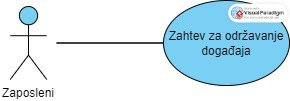
\includegraphics[scale=0.5]{Korisnici/Udruzenje/UML/SlucajUpotrebe_OdrzavanjeDogadjaja.jpeg}
    \end{center}
\caption{Dijagram za održavanje dogadjaja.}
\end{figure}

\newpage
\subsubsection{Slučaj upotrebe: Zahtev za prisustvo događaju}
\begin{enumerate}
    \item \textbf{Kratak opis:} Zaposleni u kompaniji šalje zahtev za prisustvo događaju organizovanom od strane već postojeće zajednice u kompaniji.
    \item \textbf{Učesnici:}
        \begin{itemize}
            \item Zaposleni
        \end{itemize}
    \item \textbf{Preduslovi:} Sistem je u funkciji. Zaposleni ima pristup internetu, sistemu.
    \item \textbf{Postuslovi:} Zaposleni se uspešno prijavio za prisustvo događaju. Vlasnik zajednice je obavešten.
    \item \textbf{Osnovni tok:}
        \begin{enumerate}
            \item Zaposleni otvara stranicu za udruženja.
            \item Sistem prikazuje listu svih postojećih udruženja
            \item Zaposleni otvara stranicu udruženja za čiji događaj je zainteresovan
            \item Zaposleni otvara stranicu svih događaja udruženja
            \item Zaposleni bira događaj kome želi da prisustvuje
            \item Zaposleni se prijavljuje za događaj pritiskom na dugme Želim da Prisustvujem
            \item Sistem prikazuje da je prijava uspešna 
        \end{enumerate}
    \item \textbf{Alternativni tokovi:}
        \begin{enumerate}
            \item \textbf{Prijave za događaj su zatvorene.} Sistem obaveštava korisnika da je prijavljivanje zatvoreno. Sistem vraća korisnika na korak (d)
        \end{enumerate}
    \item \textbf{Podtokovi:} /
    \item \textbf{Specijalni zahtevi:} /
    \item \textbf{Dodatne informacije:} /
\end{enumerate}

\begin{figure} [!ht]
    \begin{center}
        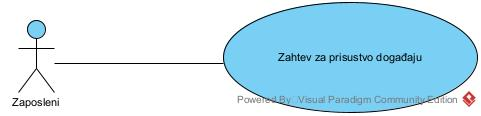
\includegraphics[scale=0.5]{Korisnici/Udruzenje/UML/SlucajUpotrebe_PrisustvoDogadjaju.jpg}
    \end{center}
\caption{Dijagram za prisustvo dogadjaju.}
\end{figure}

\end{document}
